\section{La Business Intelligence}
Inizialmente \textbf{l’informatica} ha avuto un ruolo assolutamente secondario, il cui compito era quello di memorizzare \textbf{dati operazionali}, ossia tutti quei dati che vengono generati e memorizzati per tenere traccia delle operazioni che vengono svolte in un’azienda. (es. registrazione di una fattura, ordine di materiale). Tali dati sono chiamati anche \textbf{dati transazionali}.

Un \textbf{sistema informativo} è tutto il patrimonio di dati e informazioni raccolto e gestito in maniera coerente da un’azienda. Nel sistema informativo rientrano non solo i DB ma anche tutte le informazioni che stanno nella testa delle persone, nei documenti cartacei, nelle e-mail che vengono scambiate ecc. Un \textbf{DataBase} è una raccolta di dati coerenti, organizzati secondo un modello e memorizzata su un supporto informatico. \textbf{ Un modello} è una collezione di concetti che viene usata per descrivere i dati. Ad esempio, se si ha un database relazionale, avrò una collezione di dati organizzata in tabelle e quindi avrò un \textbf{DBMS relazionale} che gestisce quel DB, dove per “gestire” si intende scrive, legge e gestisce gli accessi degli utenti a questi dati. Nei DB quando si deve fare un’operazione, nello specifico facciamo riferimento ad una \textbf{transazione}, ovvero un insieme di operazioni elementari che non possono essere fatte singolarmente, in quando le transazioni sono da considerarsi azioni atomiche. Con il passare degli anni i sistemi informativi si sono trasformati da semplici strumenti per migliorare l’efficienza dei processi, cioè più veloci, a elementi centrali dell’organizzazione aziendale, creando di per sé una ricchezza e influenzando il modo in cui fare business.
\begin{figure}[H]
	\centering
	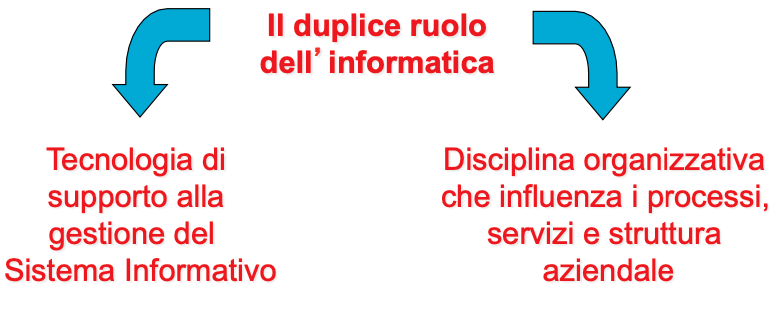
\includegraphics[width=0.9\textwidth]{img/Cursor_e_2-IntroDW_pdf}
	\caption{Ruolo dell'informatica}
	\label{fig:cursore2-introdwpdf}
\end{figure}

In questo corso, affronteremo in modo particolare il \textbf{processo decisionale}, in quando ci collochiamo ad un livello alto dell’organigramma. A noi non interessano gli impiegati, ovvero il livello medio-basso, ma i manager, cioè coloro che nell’azienda devono prendere decisioni. Nel processo decisionale il ruolo dell’informatica diventa ancora più importante. Per esempio, nel caso in cui un’azienda (Fiat o Lamborghini), volesse aprire un nuovo stabilimento bisognerebbe prendere una decisione basata sul \textbf{data driven} (guidata dai dati). Di conseguenza ho bisogno di un sistema informatico che mi aiuti nel processo decisionale.

\begin{figure}[H]
	\centering
	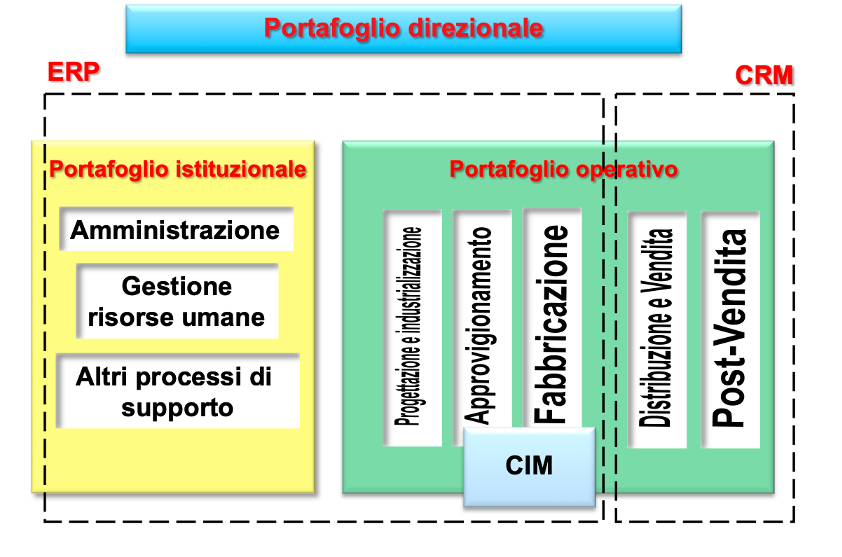
\includegraphics[width=0.7\textwidth]{img/portafoglio}
	\caption{Portafoglio Direzionale}
	\label{fig:portafoglio}
\end{figure}
Il \textbf{portafoglio direzionale} rappresentato in figura \ref{fig:portafoglio} è l’insieme delle applicazioni utilizzate dai manager aziendali per:
\begin{itemize}
	\item 
	Analizzare lo stato dell’azienda
	\item 
	Prendere decisioni rapide
	\item 
	Prendere le decisioni migliori
\end{itemize}
ed è costituito da due parti:
\begin{enumerate}
	\item 
	\textbf{ERP (Enterprise Resource Planning)}: non sono un DBMS pur gestendo dati. Coprono un’area molto vasta del business aziendali, come quella del portafoglio istituzionale e parte del portafoglio operativo e hanno caratteristiche particolari come:
	\begin{itemize}
		\item
		l’unicità del dato
		\item 
		concetto di configurazione, che permette di adattarsi in parte ai 
		requisiti della specifica azienda
		\item 
		modularità, compro solo alcuni moduli dell’ERP
	\end{itemize}
	
	Uno degli ERP più noti è \textbf{SAP}.
	
	\item 
	\textbf{CRM (customer relationship manager)}: simile all’ERP ma in ambito diverso, è più orientato al cliente. Il caso più banale è quello degli operatori telefonici che per proporre delle offerte hanno sotto un CRM, il quale indica i potenziali clienti. 
	
\end{enumerate}
Tutta la parte sotto la linea tratteggiata sono dati operazionali, i quali saranno il nostro punto di partenza.

Tipicamente si parla anche di piattaforma di \textbf{Business Intelligence}, ovvero un insieme di strumenti e procedure che consentono a un’azienda di trasformare i propri dati di business in informazioni e conoscenza utili al processo decisionale. L'\textbf{informazione} è una specie di distillato dei dati, perché abbiamo una maggiore qualità dei dati, gli errori sono stati corretti e  si è rinunciato ad un livello di dettaglio che magari non interessava per il processo decisionale. La \textbf{conoscenza}, quantità ancora minore ma valore ancora più elevato, perché a partire dalla conoscenza si possono prendere decisioni e quindi agire all’interno dell’azienda. Informazione e conoscenza vengono affidate ai decisori aziendali per decidere quali strategie adottare per il business. L’obiettivo è trarre vantaggio rispetto ai \textbf{competitor}, migliorare le prestazioni, aumentare la \textbf{profitability}, e più in generale, \textbf{creare valore} per l’azienda.
Si parla di piattaforma di BI poiché per consentire ai manager analisi potenti e flessibili è necessario definire un’apposita infrastruttura hardware e software di supporto composta da:
\begin{itemize}
	\item 
	Hardware dedicato, avrò un server su cui gira tutta la "roba" della BI
	\item 
	Infrastrutture di rete
	\item 
	DBMS, fatto in modo da gestire grandi quantità di dati
	\item 
	Software di back-end
	\item 
	Software di front-end
\end{itemize}
Il ruolo chiave di una piattaforma di BI è la trasformazione dei dati in informazioni e quindi in conoscenza.

\subsection{La piramide della BI}

\begin{figure}[H]	
	\centering
	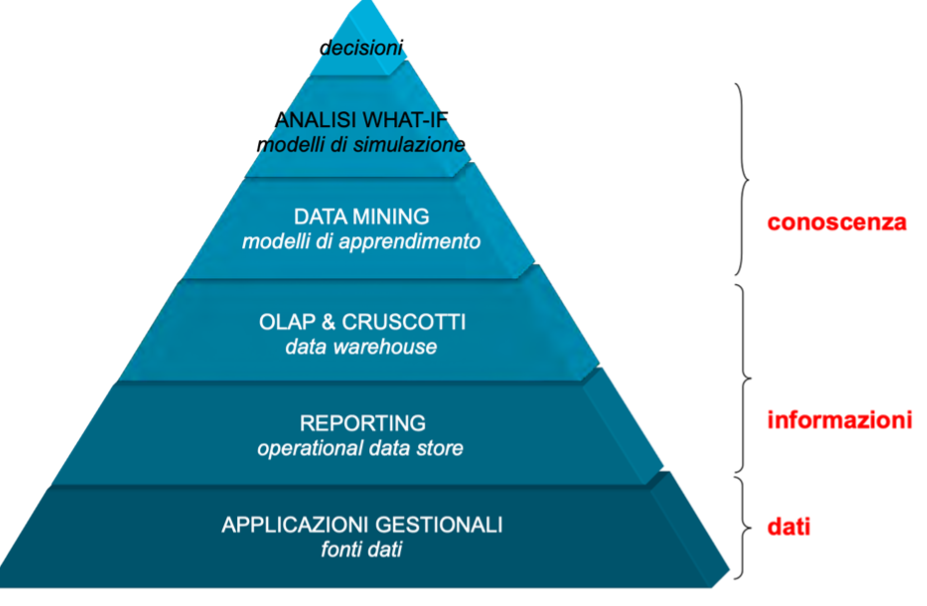
\includegraphics[width=0.7\linewidth]{img/piramide}
	\caption{Piramide della BI}
	\label{fig:piramide}
\end{figure}

Al livello più basso della piramide rappresentata in figura \ref{fig:piramide} troviamo i dati gestiti da applicazioni gestionali, cioè programmi. Per fare un esempio immaginiamo di essere un’azienda a cui serve un programma per fare le fatture in forma digitale, quindi usando un DB. I DB sappiamo che sono gestiti da un DBMS, ma non posso immaginare di fare interagire l’utente finale direttamente con un DBMS. Dunque, tra l’utente e il DBMS ho bisogno di uno strato applicativo che da un lato deve presentare delle finestre adatte ad un utente non tecnico e dall’altro deve essere in grado di parlare con il DBMS. 
Con i due livelli successivi entriamo nel mondo dell’informazione, in cui troviamo “l\textbf{’operational data store}” e il “\textbf{data warehouse}”. Il primo è un livello di database intermedio tra i due mondi, nel quale si trovano  dati dettagliati ma puliti. Nel secondo invece, ho proprio l’informazione, quindi vado ad effettuare la sintesi dei dati.

\textbf{L’operation data store}, in genere, lo uso per fare il reporting operativo, cioè per lanciare delle query che generano i cosiddetti “listoni”. Il livello di data warehouse è un repository, di natura completamente diversa rispetto a quello precedente, in cui l’interazione avviene attraverso un particolare paradigma di interrogazione, \textit{OLAP} e \textit{CRUSCOTTI} dashboard. Al livello del \textbf{DATA MINING}, si entra nel mondo della conoscenza. Gli strumenti di data mining implementano degli algoritmi complessi, in grado di estrarre conoscenza nascosta, in grosse quantità di dati, i cosiddetti pattern, ovvero schemi di comportamento che gli algoritmi di data mining riescono a portare alla luce. In particolare, tali algoritmi fanno uso delle regole associative. Ancora più in alto, troviamo l’\textbf{analisi what-if} (cosa-se). Ci si trova vicino alla cima, in cui sono presenti le decisioni. Se ho uno strumento che mi permette di prevedere, nel caso dell’esempio degli spinaci (offerta 3X2), se ci guadagno o ci perdo prendere una decisione diventa facile. Tutto ciò non è semplice da ottenere perché ci sono tanti fattori. 

Il \textbf{ciclo decisionale} in BI si articola in quattro fasi:
\begin{itemize}
	\item 
	\textbf{Analisi}: identificazione il problema e ottenere dai dati le informazioni
	\item
	\textbf{Comprensione}: analisi what-if e trasformare le informazioni in conoscenza
	\item 
	\textbf{Decisione}: traduco la conoscenza in decisioni e quindi in azioni
	\item 
	\textbf{Misura}: misurare che le prestazioni che ottengo sono in linea con le mie previsioni
\end{itemize}

Per fare tutto ciò ho bisogno di:
\begin{itemize}
	\item 
	\textbf{Tecnologie}: potenza di calcolo, tecniche avanzate di visualizzazione, capacità di memorizzazione grandi moli di dati, connettività di rete, interoperabilità software (DBMS, front-end, back-end che cooperano tra di loro)
	\item
	\textbf{Metodologie analitiche}: modelli matematici espressivi, precisi e flessibili oltre che tecniche di apprendimento induttivo e di ottimizzazione
	\item 
	\textbf{Risorse umane}: cultura aziendale, creatività, agilità mentale, disponibilità al cambiamento
	
\end{itemize}
